% ============================================================
% FEE3411 Control Systems A -- Assignment 1
% Covers: Week 1 (components and devices) + Week 2 (modelling)
% Issued Week 1, due Week 3. Worth 1.5% of the unit.
%
% ONE source, TWO outputs. The toggle keys on \jobname, so the
% student sheet and the marking scheme cannot drift apart:
%
%   latexmk -pdf -jobname=assignment-1-questions       assignment-1.tex
%   latexmk -pdf -jobname=assignment-1-marking-scheme  assignment-1.tex
%
% NB: the toggle uses the expl3 string test, not xstring's \IfSubStr --
% \jobname yields catcode-12 characters and \IfSubStr silently fails.
%
% Needs: ../tex/preamble.tex (this file lives in Assignments/).
% ============================================================
\documentclass[11pt,a4paper]{article}
\usepackage[margin=25mm]{geometry}
% ============================================================
% FEE3411 Control Systems A -- shared preamble
% Used by both the lecture notes (article) and the slides (beamer).
% ============================================================
\usepackage[T1]{fontenc}
% lmodern gives cleaner PDF fonts but is absent from minimal TeX installs.
% Load it only if present, so this preamble builds anywhere.
\IfFileExists{lmodern.sty}{\usepackage{lmodern}}{}
\usepackage{amsmath,amssymb,amsthm}
\usepackage{graphicx}
\usepackage{booktabs}
\usepackage{siunitx}
\usepackage{tikz}
\usepackage{circuitikz}
\usepackage{pgfplots}
\pgfplotsset{compat=1.18}
\usetikzlibrary{arrows.meta,positioning,calc,decorations.markings,shapes.geometric}
\usepackage[most]{tcolorbox}
\usepackage{xcolor}

% ---- Course colours -------------------------------------------------
\definecolor{fnavy}{HTML}{1F3864}
\definecolor{faccent}{HTML}{2E5E4E}
\definecolor{fflag}{HTML}{9C4221}

% ---- Block-diagram style --------------------------------------------
\tikzset{
  block/.style   = {draw, thick, rectangle, minimum height=2.6em,
                    minimum width=3.2em, align=center},
  sumnode/.style = {draw, thick, circle, inner sep=0pt, minimum size=1.6em},
  pickoff/.style = {fill, circle, inner sep=0pt, minimum size=3pt},
  sig/.style     = {-{Latex[length=2mm]}, thick},
}

% ---- Summing-junction signs -----------------------------------------
% \sumsign{<node>}{<angle>}{<+ or ->} places a sign just outside the circle.
\newcommand{\sumsign}[3]{\node[font=\small] at ($(#1)+(#2:0.5)$) {$#3$};}

% ---- Boxed environments ---------------------------------------------
\newtcolorbox{keyidea}[1][]{colback=fnavy!5,colframe=fnavy,
  fonttitle=\bfseries,title=Key idea,#1}
\newtcolorbox{workedex}[1][]{colback=faccent!5,colframe=faccent,
  fonttitle=\bfseries,title=Worked example,#1}
\newtcolorbox{pitfall}[1][]{colback=fflag!5,colframe=fflag,
  fonttitle=\bfseries,title=Common pitfall,#1}

% ---- Shorthands ------------------------------------------------------
\newcommand{\Lap}{\mathcal{L}}
\newcommand{\jw}{\mathrm{j}\omega}
\newcommand{\wn}{\omega_{n}}
\newcommand{\zt}{\zeta}
\newcommand{\TF}[1]{#1(s)}

% ---- Week title machinery -------------------------------------------
\usepackage{fancyhdr}
\newcommand{\thecoursecode}{FEE3411}
\newcommand{\thecoursename}{Control Systems A}
\newcommand{\wknum}{}
\newcommand{\wktopic}{}
\newcommand{\weeknumber}[1]{\renewcommand{\wknum}{#1}}
\newcommand{\weektopic}[1]{\renewcommand{\wktopic}{#1}}
\newcommand{\weektitle}{%
  \thispagestyle{plain}%
  \begin{center}
    {\large\sffamily\bfseries\color{fnavy}\thecoursecode: \thecoursename}\\[2pt]
    {\Huge\sffamily\bfseries Week \wknum}\\[4pt]
    {\LARGE\sffamily\color{fnavy}\wktopic}\\[6pt]
    \rule{\textwidth}{1.2pt}
  \end{center}\vspace{4pt}%
  \pagestyle{fancy}\fancyhf{}%
  \fancyhead[L]{\footnotesize\color{gray}\thecoursecode\ Week \wknum\ --- \wktopic}%
  \fancyhead[R]{\footnotesize\color{gray}\thepage}%
  \renewcommand{\headrulewidth}{0.4pt}%
}

% ---- Outcomes and reading boxes -------------------------------------
\newenvironment{outcomes}
  {\begin{tcolorbox}[colback=white,colframe=fnavy!60,
      fonttitle=\bfseries,title=By the end of this week you should be able to]
   \begin{itemize}[leftmargin=*]}
  {\end{itemize}\end{tcolorbox}}

\newtcolorbox{readingbox}{colback=gray!5,colframe=gray!50,
  fonttitle=\bfseries,title=Reading}

% enumitem must NOT be loaded under beamer: it overwrites beamer's itemize
% templates and the bullet markers silently disappear. The notes (article) get
% it; the slides (beamer) use beamer's own list machinery instead.
\makeatletter
\@ifclassloaded{beamer}{}{\usepackage{enumitem}}
\makeatother

\usepackage{environ}

% ---- marking-scheme toggle ------------------------------------------
\newif\ifscheme
\ExplSyntaxOn
\tl_set:Nx \l_tmpa_tl { \jobname }
\str_if_in:NnTF \l_tmpa_tl { marking } { \schemetrue } { \schemefalse }
\ExplSyntaxOff

\newtcolorbox{modelbox}[1][]{colback=faccent!4,colframe=faccent!70,
  fonttitle=\bfseries,title=Model answer and mark allocation,breakable,#1}
\newtcolorbox{markernote}[1][]{colback=fflag!4,colframe=fflag!70,
  fonttitle=\bfseries,title=Marker's note,breakable,#1}
\NewEnviron{scheme}{\ifscheme\begin{modelbox}\BODY\end{modelbox}\fi}
\NewEnviron{markernotes}{\ifscheme\begin{markernote}\BODY\end{markernote}\fi}

% ---- mark tags -------------------------------------------------------
% pluralises, and \mbox stops "[3" and "marks]" splitting across a line break
\newcommand{\qmarks}[1]{\hfill\mbox{\small\color{fnavy}\textbf{[#1 mark\ifnum#1=1\else s\fi]}}}
\newcommand{\mk}[1]{{\small\color{faccent}\textbf{(#1)}}}

\weeknumber{1}
\weektopic{Assignment 1 --- Components, Devices and Modelling}

\begin{document}
\weektitle

\begin{center}
\ifscheme
  {\large\sffamily\bfseries\color{fflag}MARKING SCHEME}\\[2pt]
  {\small\itshape Instructor copy. Not for circulation.}
\else
  {\large\sffamily\bfseries\color{fnavy}ASSIGNMENT 1}
\fi
\end{center}

\bigskip
\begin{readingbox}
\textbf{Issued} Week 1. \qquad
\textbf{Due} at the start of the Week 3 lecture. \qquad
\textbf{Weight} 1.5\% of the unit. \qquad
\textbf{Total} 40 marks.

\smallskip
\textbf{Covers} Week 1 (control system components and devices) and Week 2
(mathematical modelling of physical systems). Questions 3 and 4 use material
from the Week 2 lecture and tutorial, so attempt them after that week.

\smallskip
\textbf{Submit} your own handwritten or typed solutions. Show your working ---
an unsupported final answer earns little credit, and a wrong answer with sound
working earns most of it. This is individual work: you may discuss the
questions with others, but what you hand in must be written by you.

\smallskip
\textbf{No software is required.} Everything here is to be done by hand.
\end{readingbox}

% ====================================================================
\section*{Question 1 --- Anatomy of a real control system \qmarks{10}}

A photovoltaic array is mounted on a single-axis tracker so that it can follow
the sun through the day. A motor drives the array about a horizontal
north--south axis; the array angle must match the sun's elevation to within a
degree or so if the energy gain over a fixed array is to be worth the cost of
the mechanism.

\begin{enumerate}[label=(\alph*)]
\item Draw a block diagram of the tracker as a closed-loop control system.
      Label the \emph{plant}, \emph{actuator}, \emph{sensor}, \emph{controller},
      \emph{reference}, \emph{disturbance} and \emph{measurement noise}, and
      state what physical quantity each signal on your diagram carries.
      \qmarks{4}

\item Is this a \emph{regulator} or a \emph{tracking} system? Justify your
      answer in one or two sentences. \qmarks{2}

\item Name one error detector and one actuator, chosen from the devices
      surveyed in Week 1, that would be suitable here. Give one reason for each
      choice. \qmarks{2}

\item An engineer proposes to remove the sensor entirely and instead drive the
      array from a clock, using an astronomical almanac to compute where the
      sun ought to be. Give one substantial argument in favour of this
      open-loop scheme and one against. \qmarks{2}
\end{enumerate}

\begin{scheme}
\textbf{(a)} \mk{4} A correct diagram in the form of Figure~1(b) of the Week 1
notes, with the blocks identified as:
\begin{itemize}
\item \textbf{Plant} --- the array and its supporting structure. Input: torque
      from the drive. Output: array tilt angle.
\item \textbf{Actuator} --- the geared motor (or hydraulic ram). Input:
      armature voltage or valve signal. Output: torque.
\item \textbf{Sensor} --- the sun sensor, or a shaft encoder / potentiometer on
      the array axis. Input: actual tilt angle (or sun position). Output: a
      voltage.
\item \textbf{Controller} --- the electronics computing drive from error.
\item \textbf{Reference} --- the demanded tilt angle, i.e.\ the sun's elevation.
\item \textbf{Disturbance} --- wind loading torque, entering at the plant input.
\item \textbf{Measurement noise} --- added to the sensor output.
\end{itemize}
\mk{2} for a correct loop topology with a summing junction and negative
feedback; \mk{1} for all seven items labelled; \mk{1} for correctly naming the
physical quantity on each signal.

\medskip
\textbf{(b)} \mk{2} A \textbf{tracking (follow-up) system}: the reference is not
constant --- the sun's elevation changes continuously through the day, and the
array is required to follow it. \mk{1} for the correct classification,
\mk{1} for a justification that turns on the reference being time-varying.

\emph{Accept} a well-argued answer that it is \emph{both}: a tracking system
over the day, but a regulator on the timescale of a wind gust. Full marks if
the reasoning is sound.

\medskip
\textbf{(c)} \mk{2} \mk{1} for a sensible error detector with a reason ---
e.g.\ a \emph{potentiometer} on the array axis (cheap, d.c.\ output, a pure
gain $K_p$, and the axis rotates through well under one revolution so the
sliding contact is acceptable); or a \emph{synchro pair} if the environment is
harsh and a sliding contact is undesirable.

\mk{1} for a sensible actuator with a reason --- e.g.\ a \emph{d.c.\
servomotor with a large gear reduction} (high torque at low speed, simple
drive, holds position); or a \emph{hydraulic ram} for a very large array
(hydraulics give far higher force density and stiffness against wind loading).

\emph{A stepper motor is also defensible} (digital, holds position, no sensor
needed) provided the student notes the skipped-step risk under wind loading.

\medskip
\textbf{(d)} \mk{2} \mk{1} each for one sound argument on each side.

\emph{For:} the sun's position is genuinely predictable to far better than a
degree from date, time and latitude, so the reference is known in advance
without measuring anything. Removing the sensor removes its cost, its noise and
a failure mode. There is nothing to mis-calibrate and no risk of the sensor
being fooled by cloud or by a bright reflection.

\emph{Against:} the scheme cannot detect or correct anything that is not in the
model --- a stiff wind deflecting the structure, backlash or wear in the gear
train, a slipped coupling, ice, or the mounting settling out of true. Any of
these produces a pointing error that the system will never know about. It is
also entirely dependent on the clock and on the installation being surveyed in
correctly.
\end{scheme}

\begin{markernotes}
Part (a) is where most of the marks are and where most students lose them ---
usually by drawing the sensor in the forward path, or by omitting the summing
junction and simply drawing a ring of blocks. Be strict about the sign on the
feedback: it must be negative.

In (d), do not require the ``correct'' answer --- there isn't one. Reward the
recognition that open loop fails on \emph{unmodelled} effects, which is the
point of the question.
\end{markernotes}

% ====================================================================
\section*{Question 2 --- Devices \qmarks{10}}

\begin{enumerate}[label=(\alph*)]
\item Explain, in your own words and with a sketch, how a synchro
      transmitter and synchro control transformer are used together as an error
      detector. Your answer should make clear what the input and output of the
      pair are, and why the output is described as a
      \emph{suppressed-carrier} signal. \qmarks{5}

\item A three-stack variable-reluctance stepper motor has 15 teeth on each
      rotor.
      \begin{enumerate}[label=(\roman*)]
      \item Calculate the step angle. \qmarks{1}
      \item How many pulses are required for one complete revolution of the
            rotor? \qmarks{1}
      \item The motor is driven at 500 pulses per second. Find the shaft speed
            in revolutions per minute. \qmarks{1}
      \end{enumerate}

\item A hydraulic linear actuator has transfer function
      $Y(s)/X(s)=K/[s(\tau s+1)]$, whereas a spring-loaded pneumatic diaphragm
      actuator has $\Delta Y(s)/\Delta P(s)=A/(Ms^{2}+fs+K)$. Explain the
      structural difference between the two --- in particular, why one contains
      a free integrator and the other does not. \qmarks{2}
\end{enumerate}

\begin{scheme}
\textbf{(a)} \mk{5}
\begin{itemize}
\item \mk{1} Construction: the transmitter is built like a small three-phase
      alternator --- three Y-connected stator coils \ang{120} apart, a
      single-coil rotor fed a.c.\ through slip rings. The control transformer is
      the same but with a \emph{cylindrical} rotor, so its air gap and output
      impedance do not change as it turns.
\item \mk{1} Operation of the transmitter: the a.c.\ rotor excitation sets up a
      flux along the rotor axis; by transformer action a voltage is induced in
      each stator coil, proportional to the cosine of the angle between that
      coil's axis and the rotor axis. Input is a shaft angle; output is three
      a.c.\ voltages encoding it.
\item \mk{1} The three stator leads feed the control transformer's stator,
      reproducing the same flux pattern there; the voltage induced in its rotor
      is proportional to the cosine of the angle between the two rotors, giving
      for small differences
      $e(t)\approx K_{s}(\theta-\alpha)\sin\omega_{c}t$.
\item \mk{1} \textbf{Input} of the pair: the \emph{difference} between two
      shaft angles. \textbf{Output}: a single a.c.\ voltage whose amplitude is
      proportional to that difference. $K_{s}$ is the sensitivity,
      \si{\volt\per\radian}.
\item \mk{1} \textbf{Suppressed carrier}: the information is carried in the
      \emph{amplitude} (the envelope) of the carrier $\sin\omega_{c}t$, and the
      \emph{phase reverses} when the error changes sign. The carrier itself
      conveys nothing; at zero error the output vanishes entirely.
\end{itemize}
A sketch resembling Figure~7 of the Week 1 notes is expected but need not be
elaborate --- two circles, three leads between the stators, rotor angles marked.

\medskip
\textbf{(b)}
\begin{enumerate}[label=(\roman*)]
\item \mk{1} $\displaystyle \alpha=\frac{360^{\circ}}{nT}
      =\frac{360^{\circ}}{3\times 15}=\ang{8}$.
\item \mk{1} $360/8=\boxed{45}$ pulses per revolution.
\item \mk{1} $\dfrac{500}{45}=11.11\ \text{rev/s}
      \;\Rightarrow\; 11.11\times 60 = \boxed{\SI{667}{rev/min}}$
      (to three significant figures).
\end{enumerate}

\medskip
\textbf{(c)} \mk{2}
\mk{1} In the hydraulic actuator, the valve opening $x$ sets the \emph{rate of
oil flow} into the cylinder, and flow rate sets the piston's \emph{velocity}
($q=A\dot y$). Position is therefore the integral of the input, which is
precisely the $1/s$. Hold the valve open and the ram keeps moving.

\mk{1} In the pneumatic actuator the diaphragm works against a \emph{return
spring}. A constant pressure produces a constant \emph{force}, which the spring
balances at a definite \emph{position}. There is nothing to integrate, so the
transfer function is a plain second-order lag with a finite d.c.\ gain $A/K$.
\end{scheme}

\begin{markernotes}
In (b)(iii), accept \SI{666.7}{rev/min} or \SI{667}{rev/min}. Deduct nothing
for the rounding, but do deduct \mk{1} if the student divides by the step angle
in degrees rather than by pulses per revolution --- a common slip that gives
$500/8=62.5$.

In (c), the answer that earns the marks is the one about \emph{rate versus
position}, not one that merely observes that ``one has an $s$ in the
denominator''. Restating the algebra is not an explanation.
\end{markernotes}

% ====================================================================
\section*{Question 3 --- Modelling two physical systems \qmarks{10}}

\begin{center}
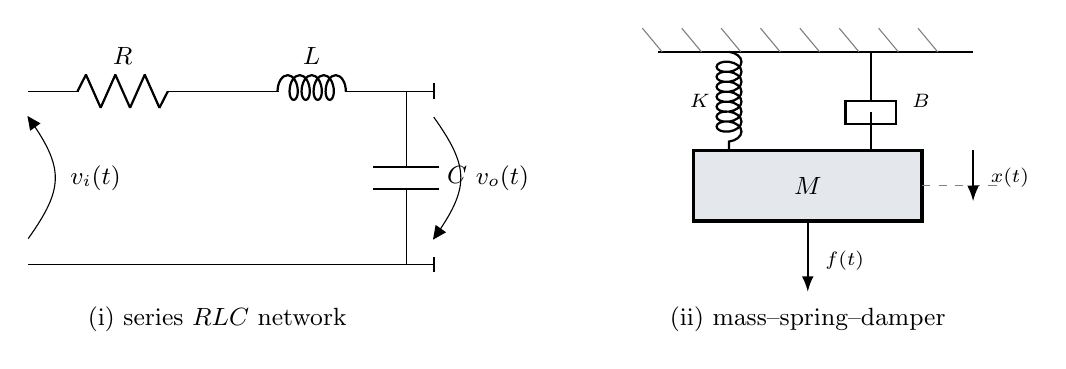
\begin{tikzpicture}[x=1cm, y=1cm, font=\small]
% ---------- (i) series RLC ----------
\begin{scope}
\draw (0,0) to[R=$R$] (2.4,0) to[L=$L$] (4.8,0);
\draw (4.8,0) to[C=$C$] (4.8,-2.2);
\draw (4.8,-2.2) -- (0,-2.2);
\draw (0,0) to[open, v^<=$v_i(t)$] (0,-2.2);
\draw[thick] (5.15,-0.1) -- (5.15,0.1);
\draw[thick] (5.15,-2.3) -- (5.15,-2.1);
\draw (4.8,0) -- (5.15,0);
\draw (4.8,-2.2) -- (5.15,-2.2);
\draw (5.15,0) to[open, v^>=$v_o(t)$] (5.15,-2.2);
\node at (2.4,-2.9) {(i) series $RLC$ network};
\end{scope}
% ---------- (ii) mass-spring-damper ----------
\begin{scope}[shift={(8.6,-0.4)}]
\draw[thick] (-0.6,0.9) -- (3.4,0.9);
\foreach \i in {0,...,7}
  \draw[gray] ({-0.55+\i*0.5},0.9) -- ({-0.8+\i*0.5},1.2);
% spring
\draw[thick, decorate, decoration={coil, aspect=0.6, segment length=3.6pt,
      amplitude=4.5pt}] (0.3,0.9) -- (0.3,-0.35);
\node[left,font=\scriptsize] at (0.18,0.28) {$K$};
% damper
\draw[thick] (2.1,0.9) -- (2.1,0.28);
\draw[thick] (1.78,0.28) rectangle (2.42,-0.02);
\draw[thick] (2.1,0.13) -- (2.1,-0.35);
\node[right,font=\scriptsize] at (2.5,0.28) {$B$};
% mass
\draw[very thick,fill=fnavy!12] (-0.15,-1.25) rectangle (2.75,-0.35);
\node at (1.3,-0.8) {$M$};
% displacement and force
\draw[sig] (1.3,-1.25) -- (1.3,-2.15);
\node[right,font=\scriptsize] at (1.4,-1.75) {$f(t)$};
\draw[dashed,gray] (2.75,-0.8) -- (3.7,-0.8);
\draw[sig] (3.4,-0.35) -- (3.4,-1.0);
\node[right,font=\scriptsize] at (3.5,-0.7) {$x(t)$};
\node at (1.3,-2.5) {(ii) mass--spring--damper};
\end{scope}
\end{tikzpicture}
\end{center}

\begin{enumerate}[label=(\alph*)]
\item For the series $RLC$ network of figure (i), with input the source voltage
      $v_{i}(t)$ and output the capacitor voltage $v_{o}(t)$:
      \begin{enumerate}[label=(\roman*)]
      \item derive the governing differential equation from first principles;
      \item hence obtain the transfer function $V_{o}(s)/V_{i}(s)$, assuming
            zero initial conditions;
      \item write down the characteristic equation, and evaluate it for
            $R=\SI{4}{\ohm}$, $L=\SI{1}{\henry}$, $C=\SI{0.125}{\farad}$.
      \end{enumerate}
      \qmarks{5}

\item For the mass--spring--damper of figure (ii), with input the applied force
      $f(t)$ and output the displacement $x(t)$, obtain the differential
      equation, the transfer function $X(s)/F(s)$ and the characteristic
      equation. Evaluate for $M=\SI{1}{\kilogram}$,
      $B=\SI{4}{\newton\second\per\metre}$, $K=\SI{8}{\newton\per\metre}$.
      \qmarks{3}

\item Compare your two characteristic equations. What does the comparison tell
      you, and what does it \emph{not} tell you? (Look also at the d.c.\ gain
      of each transfer function.) \qmarks{2}
\end{enumerate}

\begin{scheme}
\textbf{(a)} \mk{5}

\emph{(i)} \mk{2} Kirchhoff's voltage law round the loop, with the same current
$i$ through all three elements:
\[
  v_{i}=Ri+L\frac{di}{dt}+v_{o},
  \qquad i=C\frac{dv_{o}}{dt}.
\]
Substituting for $i$:
\[
  \boxed{\;LC\,\ddot v_{o}+RC\,\dot v_{o}+v_{o}=v_{i}\;}
\]
\mk{1} for KVL correctly applied, \mk{1} for eliminating $i$ correctly.

\emph{(ii)} \mk{2} Transforming with zero initial conditions:
\[
  \left(LCs^{2}+RCs+1\right)V_{o}(s)=V_{i}(s)
  \qquad\Longrightarrow\qquad
  \frac{V_{o}(s)}{V_{i}(s)}=\frac{1}{LCs^{2}+RCs+1}.
\]

\emph{(iii)} \mk{1} Characteristic equation $LCs^{2}+RCs+1=0$. With the given
values $LC=0.125$, $RC=0.5$:
\[
  0.125s^{2}+0.5s+1=0
  \quad\Longleftrightarrow\quad
  \boxed{\;s^{2}+4s+8=0\;}
\]
and the transfer function is $8/(s^{2}+4s+8)$, of d.c.\ gain $8/8=1$.
Roots $s=-2\pm j2$.

\medskip
\textbf{(b)} \mk{3} Newton's second law on the mass, taking $x$ positive in the
direction of $f$, with the spring and damper both opposing motion:
\[
  M\ddot x = f - B\dot x - Kx
  \qquad\Longrightarrow\qquad
  \boxed{\;M\ddot x+B\dot x+Kx=f\;}
\]
\[
  \frac{X(s)}{F(s)}=\frac{1}{Ms^{2}+Bs+K},
  \qquad\text{characteristic equation } Ms^{2}+Bs+K=0 .
\]
With the given values:
\[
  \boxed{\;s^{2}+4s+8=0\;}
  \qquad\text{and}\qquad
  \frac{X(s)}{F(s)}=\frac{1}{s^{2}+4s+8},
  \quad\text{d.c.\ gain }\tfrac{1}{8}.
\]
\mk{1} free-body/force balance, \mk{1} transfer function, \mk{1} numerical
characteristic equation.

\medskip
\textbf{(c)} \mk{2}

\mk{1} \emph{What it tells you.} The two characteristic equations are
\textbf{identical}: $s^{2}+4s+8=0$, roots $s=-2\pm j2$. The two systems ---
one electrical, one mechanical --- therefore have exactly the same
\emph{dynamic behaviour}: the same natural frequency
$\wn=\sqrt{8}=\SI{2.83}{\radian\per\second}$, the same damping ratio
$\zt=4/(2\sqrt 8)=0.707$, the same transient shape
$e^{-2t}(\ldots\cos 2t\ldots\sin 2t)$, the same settling time. This is the
\emph{force--voltage analogy}: $M\leftrightarrow L$,
$B\leftrightarrow R$, $K\leftrightarrow 1/C$. It is why one body of
mathematics serves every branch of engineering, and why we shall spend the rest
of this unit studying $s^{2}+2\zt\wn s+\wn^{2}$ rather than studying circuits
and masses separately.

\mk{1} \emph{What it does not tell you.} The characteristic equation says
nothing about the \emph{gain}. The electrical system has d.c.\ gain 1
(\si{\volt\per\volt}); the mechanical one has d.c.\ gain $1/8$
(\si{\metre\per\newton}). Same dynamics, different scale --- and different
units entirely. Nor does it say anything about what the input and output
physically are.

\emph{Bonus observation, not required for marks:} this is the same
characteristic equation as the position servo in Question 5 of the Week 1
tutorial.
\end{scheme}

\begin{markernotes}
Sign errors in (b) are the usual loss. The spring and damper forces
\emph{oppose} the motion, so they appear on the opposite side of Newton's law
from $f$; a student who writes $M\ddot x+B\dot x+Kx=-f$ or
$M\ddot x=f+B\dot x+Kx$ has the physics wrong, not merely the algebra ---
deduct the \mk{1} for the force balance but allow the remaining marks to follow
through their (incorrect) equation.

Part (c) separates the students who have understood the week from those who
have executed it. Award the second mark only for an answer that identifies
\emph{gain} (or units, or scale) as the thing the characteristic equation
misses. ``It doesn't tell you the input'' alone is too vague.
\end{markernotes}

% ====================================================================
\section*{Question 4 --- The armature-controlled d.c.\ servomotor \qmarks{10}}

An armature-controlled d.c.\ servomotor has armature resistance $R_{a}$ and
inductance $L_{a}$, torque constant $K_{t}$ and back-emf constant $K_{b}$. Its
rotor has moment of inertia $J_{m}$ and viscous friction coefficient $b$. The
input is the armature voltage $v_{a}(t)$; the field is separately excited and
held constant.

\begin{enumerate}[label=(\alph*)]
\item Write down the armature circuit equation and the mechanical (torque
      balance) equation. Define every symbol you use, and state clearly the two
      assumptions that make this a \emph{linear} model. \qmarks{3}

\item Eliminating the armature current, derive the transfer function
      $\theta_{m}(s)/V_{a}(s)$. \qmarks{3}

\item Show that when the armature inductance is negligible, $L_{a}\to 0$, the
      result takes the form
      \[
        \frac{\theta_{m}(s)}{V_{a}(s)}=\frac{K_{m}}{s(\tau_{m}s+1)},
      \]
      and give $K_{m}$ and $\tau_{m}$ in terms of the motor parameters.
      Evaluate both for $R_{a}=\SI{2}{\ohm}$,
      $K_{t}=\SI{0.5}{\newton\metre\per\ampere}$,
      $K_{b}=\SI{0.5}{\volt\second\per\radian}$,
      $J_{m}=\SI{0.02}{\kilogram\metre\squared}$ and
      $b=\SI{0.01}{\newton\metre\second\per\radian}$. \qmarks{2}

\item The motor now drives a load of inertia
      $J_{L}=\SI{1.5}{\kilogram\metre\squared}$ through a gear train of ratio
      $n=\theta_{L}/\theta_{m}=1/10$. Explain how the load inertia appears at
      the motor shaft, recompute $\tau_{m}$, and comment on the result. Load
      friction may be neglected. \qmarks{2}
\end{enumerate}

\begin{scheme}
\textbf{(a)} \mk{3}

\emph{Armature circuit} (KVL), \mk{1}:
\[
  v_{a}=R_{a}i_{a}+L_{a}\frac{di_{a}}{dt}+e_{b},
  \qquad e_{b}=K_{b}\frac{d\theta_{m}}{dt}
\]
where $e_{b}$ is the back emf, proportional to shaft speed.

\emph{Mechanical} (Newton's second law for rotation), \mk{1}:
\[
  T_{m}=K_{t}i_{a}=J_{m}\frac{d^{2}\theta_{m}}{dt^{2}}
        +b\frac{d\theta_{m}}{dt}
\]
with $T_{m}$ the developed torque, proportional to armature current.

\emph{Assumptions}, \mk{1} (both needed):
\begin{enumerate}[label=(\roman*)]
\item The field flux is \textbf{constant}. Torque is in general proportional to
      the product of flux and armature current; holding the flux fixed makes
      $T_{m}=K_{t}i_{a}$ \emph{linear}. (Equivalently: the magnetic circuit is
      unsaturated.)
\item Friction is \textbf{purely viscous}, i.e.\ proportional to speed.
      Coulomb friction and stiction are neglected --- they are not linear and
      would put a dead zone at low speed.
\end{enumerate}
\emph{Also accept:} negligible backlash in the coupling; brush contact drop
neglected; armature parameters constant with temperature.

\medskip
\textbf{(b)} \mk{3} Transforming both equations with zero initial conditions:
\[
  V_{a}(s)=(R_{a}+L_{a}s)I_{a}(s)+K_{b}s\,\theta_{m}(s),
  \qquad
  K_{t}I_{a}(s)=(J_{m}s^{2}+bs)\,\theta_{m}(s).
\]
\mk{1} for both transforms. From the second,
$I_{a}=(J_{m}s^{2}+bs)\theta_{m}/K_{t}$ \mk{1}; substituting into the first,
\[
  V_{a}=\frac{(R_{a}+L_{a}s)(J_{m}s^{2}+bs)}{K_{t}}\theta_{m}+K_{b}s\theta_{m}
\]
\[
  \boxed{\;\frac{\theta_{m}(s)}{V_{a}(s)}
   =\frac{K_{t}}{s\left[(R_{a}+L_{a}s)(J_{m}s+b)+K_{t}K_{b}\right]}\;}
  \qquad \mk{1}
\]
Note the free $s$ in the denominator, which has been factored out of
$J_{m}s^{2}+bs$: the motor is an \emph{integrator}, because a constant voltage
gives a constant \emph{speed}, and position is the integral of speed.

\medskip
\textbf{(c)} \mk{2} Setting $L_{a}=0$:
\[
  \frac{\theta_{m}}{V_{a}}
   =\frac{K_{t}}{s\left[R_{a}(J_{m}s+b)+K_{t}K_{b}\right]}
   =\frac{K_{t}/(R_{a}b+K_{t}K_{b})}
         {s\left[\dfrac{J_{m}R_{a}}{R_{a}b+K_{t}K_{b}}s+1\right]}
\]
\[
  \boxed{\;K_{m}=\frac{K_{t}}{R_{a}b+K_{t}K_{b}},
  \qquad
  \tau_{m}=\frac{J_{m}R_{a}}{R_{a}b+K_{t}K_{b}}\;}
  \qquad \mk{1}
\]
Numerically, $R_{a}b+K_{t}K_{b}=(2)(0.01)+(0.5)(0.5)=0.02+0.25=0.27$, so
\[
  K_{m}=\frac{0.5}{0.27}=\SI{1.85}{\radian\per\volt\per\second},
  \qquad
  \tau_{m}=\frac{(0.02)(2)}{0.27}=\SI{0.148}{\second}.
  \qquad \mk{1}
\]

\emph{Worth noticing:} $K_{t}K_{b}=0.25$ dwarfs $R_{a}b=0.02$. The motor's own
back emf, not its bearing friction, supplies almost all of the damping. This is
the electromechanical version of the point made about the a.c.\ servomotor in
Week 1.

\medskip
\textbf{(d)} \mk{2}

\mk{1} \emph{Reflection.} Through a gear train of ratio
$n=\theta_{L}/\theta_{m}$, the load turns $n$ times as far as the motor, so
kinetic energy equality (or torque balance) gives an equivalent inertia at the
\emph{motor} shaft of
\[
  J_{\text{eq}}=J_{m}+n^{2}J_{L}.
\]
The $n^{2}$ is the essential point: the gearing scales inertia by the
\emph{square} of the ratio, which is exactly why a reduction gear lets a small
low-inertia motor drive a large load.

\mk{1} \emph{Numerically:}
\[
  J_{\text{eq}}=0.02+\left(\tfrac{1}{10}\right)^{2}(1.5)
   =0.02+0.015=\SI{0.035}{\kilogram\metre\squared},
\]
\[
  \tau_{m}'=\frac{J_{\text{eq}}R_{a}}{R_{a}b+K_{t}K_{b}}
   =\frac{(0.035)(2)}{0.27}=\SI{0.259}{\second}.
\]
\emph{Comment:} the time constant rises by a factor of $1.75$ --- the loaded
servo is markedly more sluggish. Note also how effective the gearing is: a load
75 times the rotor's own inertia adds only about three quarters as much again
at the motor shaft, because $n^{2}=1/100$. Without the gearing
($n=1$) the equivalent inertia would be $\SI{1.52}{\kilogram\metre\squared}$
and $\tau_{m}$ about \SI{11}{\second} --- useless for a servo.
\end{scheme}

\begin{markernotes}
Part (b) is standard bookwork and should be marked strictly: the three marks
are for the two transforms, the elimination, and the final expression with the
$s$ correctly factored out.

The commonest error in (d) is by far $J_{\text{eq}}=J_{m}+nJ_{L}$ --- the
$n^{2}$ forgotten. Deduct the reflection mark but follow through on the
arithmetic. The second commonest is inverting the ratio, giving
$J_{\text{eq}}=0.02+100(1.5)$; that produces an absurd \SI{1111}{\second} time
constant, so a student who reports it without comment has stopped thinking
about whether the answer is physical. Note it on the script.

Do not require the closing comment in (d) for the marks, but flag good ones ---
students who spot why gearing is used at all have understood something the
question only hinted at.
\end{markernotes}

% ====================================================================
\vfill
\begin{center}
\rule{0.5\textwidth}{0.4pt}\\[4pt]
{\small\itshape
\ifscheme
  End of marking scheme. Total 40 marks, scaled to 1.5\% of the unit.
\else
  End of Assignment 1. Total 40 marks.\\
  Due at the start of the Week 3 lecture.
\fi}
\end{center}

\end{document}
